\documentclass[letterpaper]{article}
\usepackage{aaai2027}
\usepackage[hyphens]{url}
\usepackage{graphicx}
\urlstyle{rm}
\def\UrlFont{\rm}
\usepackage{natbib}
\usepackage{caption}
\frenchspacing
\usepackage{booktabs}
\pdfinfo{
/TemplateVersion (2027.1)
}
\setcounter{secnumdepth}{0}


\title{Repair Without Stopping: A Runtime for Online Evolution\\of Hybrid Code--VLA Robot Programs (Student Abstract)}
\author{
    Chukwuemeka Samuel Udoh
}
\affiliations{
    Ashesi University, 1 University Avenue, Berekuso, Ghana\\
    +234 707 209 9407, udoh.emeka@ashesi.edu.gh, https://udohchuks.github.io/
}

\begin{document}

\maketitle

\begin{abstract}
Coding agents can write and revise robot programs, and vision-language-action (VLA) models handle the contact-rich steps that code does poorly. In current hybrid programs, fixing a skill during deployment means restarting the task. We present a runtime that lets an agent repair skills while the task runs. A Rust loop plays robot actions at a fixed rate. A Python core hosts the skills, which can be replaced live and rolled back if they fail, using the revertible effects of Cordis. In simulation, with a scripted placeholder for the VLA, the control loop kept its timing while Python stalled for up to 2.7\,s. The runtime rejected or rolled back all 80 broken repairs without a restart, and an LLM's first repair was kept in 25 of 25 sessions. On a physics-simulated SO-101 arm, a halt enforced in Rust prevented contact with a bowl in 10 of 10 runs; without it, the arm hit the bowl every time.
\end{abstract}

\begin{figure*}[t]
\centering
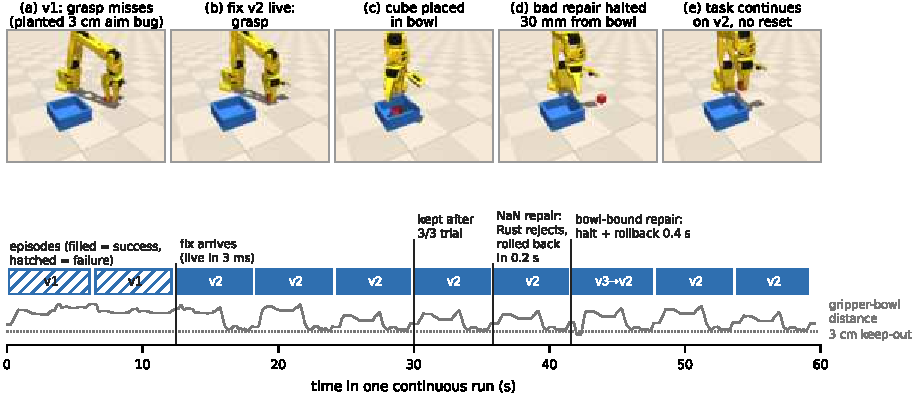
\includegraphics[width=\textwidth]{fig_mujoco_demo.pdf}
\caption{One continuous 60\,s run on the MuJoCo SO-101 arm. Top: frames. Bottom: episodes (filled = success) and repair events; v3$\rightarrow$v2 = bad repair removed mid-episode; dotted line = 3\,cm safety zone, active only during approach. The robot is never reset.}
\label{fig:demo}
\end{figure*}

\section{Introduction}
Coding agents write robot programs as readable skills that keep state and can be fixed one at a time \cite{liang2023cap,fu2026capx}. Code skills struggle in contact-rich steps, where VLA models do better \cite{shukor2025smolvla}, and hybrid systems such as SkipVLA \cite{agrawal2026skipvla} combine both. Once such a program is deployed, however, fixing a skill usually means restarting it. Dynamic software updating can replace code while it runs, in general software and in robots \cite{hayden2012kitsune,elyaacoub2023dsu}. A robot also needs a bad replacement to be rolled back, and the commands it has already sent to the arm to be cancelled. We study this combination as an online improvement loop. While the task runs, each repair is tried, then kept or rolled back, so the program improves without a human in the loop. ``Without stopping'' means the runtime is never restarted; the arm may still hold safely. We target robots that run the VLA on their own computer, where a restart means reloading model weights. Figures, tables and extra results are in the supplement.

\section{Runtime Design}
\begin{figure}[t]
\centering
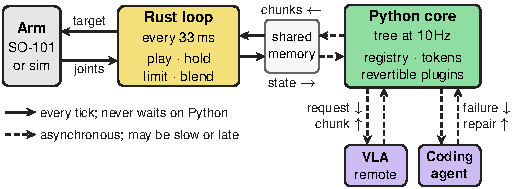
\includegraphics[width=0.85\columnwidth]{fig_arch.pdf}
\caption{Runtime architecture.}
\label{fig:arch}
\end{figure}

\textbf{Live loop (Rust).} Python cannot hold a fixed rate. VLA inference or agent calls can take seconds, and one call that holds Python's global lock freezes every Python thread. A separate Rust process (Fig.~\ref{fig:arch}) therefore runs a 30\,Hz loop; each step is a tick. Commands arrive as chunks, short lists of up to 50 target poses, stamped with the tick at which the first should play. Rust plays one action per tick and skips actions whose tick has passed. A new chunk replaces what is left of the old one. Rust rejects non-finite values and caps speed and acceleration. If Python's heartbeat stops for 200\,ms, Rust plays at most 10 more actions, then holds.

\textbf{Skills and ownership (Python).} The task is a behavior tree \cite{colledanchise2018bt} stepped at 10\,Hz. Each leaf is a node, either a code skill or the VLA, and drives the arm by sending chunks. One node drives at a time. Each time a node starts driving, it gets a new ID (a token) stamped on its chunks. To stop a node, Python asks Rust to halt its token. Rust drops every waiting or playing chunk with that token or an older one, then brings the arm to rest. The runtime requests the halt when a node is replaced, throws an error, or one call runs over 0.5\,s.

\textbf{Repairs that can be undone.} Skills are plugins. As in Cordis \cite{shi2026cordis}, each step a plugin takes while loading comes with a matching undo. If loading crashes, the undos run newest-first. A repair (new skill version) loads beside the old one. It takes over only when the old version is idle, with no chunks waiting or playing. It is kept only if the next 3 episodes succeed, which we call its trial; otherwise the old version comes back.

\section{Preliminary Validation}
\textbf{Kinematic tests.} We used two 2-core machines without GPU, a cloud VM and a laptop VM, and a simple pick-and-place simulator (hand, cube, bowl). We stalled Python with VLA delays up to 2\,s, a call that held the global lock for up to 2.7\,s, a skill that throws errors, and killing Python. Rust kept sending commands in every condition; on the cloud VM, 20 of 34{,}362 ticks ran over one period late. Inline and threaded Python-only loops froze for up to 2.3\,s. A hand-written fix for a buggy skill took over in 198\,ms. A restart with SmolVLA loaded took about 20\,s. We loaded 10 kinds of faulty repair, 10 times each; all 80 broken ones were rejected or rolled back, and Rust never played an action from a halted token. With a plain hot reload, six broken kinds stayed live and none of their 90 later episodes succeeded.

\textbf{Repairs written by an LLM.} We planted one of five simple bugs in the approach skill, such as a flipped sign. After two failed episodes, DeepSeek-V4.1-Flash received the skill's code, the plugin API and a report of observed poses. In 25/25 sessions its first answer was kept, 22--66\,s after the report, while episodes kept running. So the improvement loop can run without a human, at least for simple bugs.

\textbf{Physics simulation.} We ran the same runtime on a MuJoCo SO-101 arm, with the cube held by friction alone. In one continuous run (Fig.~\ref{fig:demo}), the fix (v2) replaced the buggy v1 and was kept. We then injected two faulty repairs. Rust rejected the first, which sent invalid numbers, before any of its actions played. The second (v3) drove toward the bowl wall. A 3\,cm safety check halted it through Rust, without contact. Both were removed, and all 8 episodes after the fix succeeded. When the arm was driven straight at the bowl, a Rust halt stopped it in 10/10 runs without contact. With no halt, or a halt only in Python, it hit the bowl in 10/10. So a halt must drop the commands already sent, in the layer that plays them.

\section{Limitations and Next Steps}
Simulation and a scripted VLA test the mechanisms, not task reliability. The bugs were planted, and the safety check reads exact distances from the simulator; on a real robot these must come from perception. A real VLA also adds slow, variable inference on the same computer. Our next step is to deploy the runtime on a real SO-101 arm.

\bibliography{refs}

\end{document}
